\documentclass[landscape]{beamer}
\usetheme{Hannover}

\usepackage{mybeamer}
\usepackage{beamerseminar}
\usepackage{hyperref}
\usepackage{multimedia}
\usepackage{graphicx}
\usepackage{comment}


\hyperbaseurl{http://www.ee.surrey.ac.uk/CVSSP/Ravl/RavlDoc/share/doc/RAVL/Auto/Basic/}

\setbeamercovered{transparent=3}

\begin{document}

\begin{frame}
  \pagecolor{titlebg} %\thispagestyle{empty}
  \begin{center}
    \huge\parbox{0.75\textwidth}{ \textcolor{titlecolor}{ \centering ~\\~Programming in C++~\\ using\\[1ex] {\Huge RAVL}\\[1em]\textcolor{royalblue}{Bill Christmas}\\[1ex]}}
  \end{center}
\end{frame}
%\pagecolor{pale}

\begin{comment}
  &&&& Things to do: more browsing actual doc at some point condense some of
  early boring stuff more actual compile & run of examples STL support now in
  (a bit) generic vector types TFVectorC & how they relate to "user" types.
\end{comment}
\section{Introduction}

\begin{frame}\frametitle{Introduction}

This presentation:

\begin{itemize}
\item includes a bit of the background to Ravl

\pause\item gives you an idea of some of the functionality available in RAVL;
  
\pause\item provides some examples of programming using RAVL;

\end{itemize}

\vfill\pause  ..... {\em not} a comprehensive tour of RAVL

\end{frame}

\begin{frame}  \frametitle{History}

  \begin{itemize}
  \item AMMA C++ library --- c.\ 1995?? --- Radek Ma\v{r}ik
\vfill\pause
  \item New version --- RAVL --- c.\ 2000 --- Charles Galambos
  \end{itemize}
  
\end{frame}

\begin{frame}  \frametitle{RAVL features}
  
  \begin{itemize}
    \pause\item  C++ class library:
    \begin{itemize}
    \item Basic containers
    \item System interface
    \item Maths, geometry inc. projective geometry - 2D \& 3D
    \item Image, video, 2D \& 3D, audio and supporting tools
    \item Pattern recognition
    \item GUIs (GTK-based)
    \item Applications (a few)
    \end{itemize} 
    
    \pause\item  Motivation: 
    \begin{itemize}
    \item lack of existing s/w (c. 1995)
    \item C++ ``difficult''
    \item explicit memory management tedious
    \end{itemize}
  
    \pause\item  Consistent programming interface 
    
    \pause\item  Not much C++ knowledge required to use it

    \pause\item  \Href{Tree/Ravl.API.Core.STL.html}{RAVL and STL}

    \pause\item  \Href{Tree/Ravl.API.Images.Converters.OpenCV.html}{RAVL and OpenCV}

  \end{itemize}
  
\end{frame}


\begin{frame}  \frametitle{Support features}

  \begin{itemize}
  \item Multi-platform:  Linux, MS, ...

  \pause\item Used for real products (Omniperception Ltd.)

  \pause\item Source code available from SourceForge, under LGPL

  \pause\item Simplified compilation system

  \pause\item Recompiled and tested nightly

  \pause\item Automatic documentation generation
    
  \pause\item Full documentation on web: \Href{http://www.ee.surrey.ac.uk/CVSSP/Ravl}{http://www.ee.surrey.ac.uk/CVSSP/Ravl}

  \pause

  \end{itemize}

\end{frame}




\section{Basics}


\begin{frame}[fragile]\frametitle{RAVL C++ basics}

  \pause\begin{itemize}
  \item \Href{Tree/Ravl.Introduction.Naming_Conventions.html}{RAVL naming conventions}
  \pause\item \Href{Class/..html}{RAVL namespaces} --- easily overlooked

  \pause\item \Href{Class/RavlN.html\#IntT}{RAVL primitive typedefs} --- for more consistent word lengths

  \pause\item RAVL constants --- under \Href{Class/RavlConstN.html}{\tt RavlConstN} namespace:

\begin{Code}
  RealT x = RavlConstN::pi; 
\end{Code}
\pause\begin{Code}
  using namespace RavlConstN;
  RealT x = pi; 
\end{Code}
  \pause\item \Href{Class/RavlN.IndexC.html}{\tt IndexC} - replacement for {\tt int} that provides more consistent rounding behaviour

  \pause\item \Href{Tree/Ravl.Introduction.Coordinate_Systems.html}{RAVL coordinates}: 
  {
\setlength{\unitlength}{3947sp}%
\begin{picture}(544,330)(376,150)
\thinlines
{\color[rgb]{0,0,0}\put(451,389){\vector( 0,-1){300}}
\put(451,389){\vector( 1, 0){300}}
}%
\put(400,-40){\rm\em x}%
\put(780,340){\rm\em y}%

\end{picture}%
}
  \end{itemize}
\end{frame}

\begin{frame}[fragile]  \frametitle{Member function syntax}

In general, C++ classes have 2 ways of accessing member functions:

\begin{itemize}
\item ``struct'' syntax:
  \begin{Code}
    a.b(); 
  \end{Code}
\item ``pointer'' syntax:
  \begin{Code}
    a->b();
  \end{Code}
  
\end{itemize}

\pause RAVL always uses the ``struct'' syntax, except where iterators are used.

\end{frame}

\begin{frame}  \frametitle{Reference counting: big / small objects}
All ``big'' objects:

\begin{itemize}
\pause\item are generally objects of indeterminate size (e.g.\ containers)
\pause\item have a \emph{handle} (a reference-counted pointer)
\pause\item identified by \Href{Class/RavlN.Array1dC.html}{inheritance of {\tt RCHandleC} or {\tt BufferAccessC}}\\ (+ StringC)
\end{itemize}

\vfill\pause ``Small'' objects behave like built-ins (int, double etc.)\vfill


    \pause{\color{blue}$\longrightarrow$} ``JAVA-like'' class interfaces\\
    \pause{\color{blue}$\longrightarrow$} (almost) no pointers\\
    \pause{\color{blue}$\longrightarrow$} automatic destruction \\
    \pause{\color{blue}$\longrightarrow$} no memory leaks (I believe)\\
    \pause{\color{blue}$\longrightarrow$} thread-safe for SMP \\
        
\end{frame}


\begin{frame}[fragile]\frametitle{Example: big object}


 Only the handle is copied in this example, \emph{not} the contents (like a ``C'' array):
  
\begin{Code}
  Array1dC<IntT>a(6);
  a.Fill(27);
  Array1dC<IntT>b = a;
  b[4] = 55;
  cout << a[4] << endl;
\end{Code}

{\footnotesize\color{xterm}$>$ myprog\\55}

\vspace{1em}

Thus the value of a[4] is also changed.


\end{frame}

\begin{frame}[fragile]\frametitle{Copying big objects}

\begin{Code}[commandchars=\\\{\}]
  Array1dC<DListC<IntT> > a(6);
  // then initialise object `a' somehow
  
  // just copies array handle:
  Array1dC<DListC<IntT> > b = a;
\end{Code}
  
  {\pause}\begin{Code}[commandchars=\\\{\}]
  // copies array of list handles:
  Array1dC<DListC<IntT> > b = a.Copy(); 
  
\end{Code}
  
  {\pause}\begin{Code}[commandchars=\\\{\}]
  // copies everything (maybe - best avoided 'til ready):
  Array1dC<DListC<IntT> > b = a.DeepCopy() 
\end{Code}

\end{frame}



\section{Base classes}


\begin{frame}[fragile]\frametitle{Text and files}

  \begin{itemize}
  \item \Href{Class/RavlN.StringC.html}{\tt StringC} - for basic text processing.  \pause E.g.:

\begin{Code}
  StringC a("Hello");  StringC b("World");
  StringC c = a + ' ' + b;
  cout << c.from('o') << endl;
\end{Code}

generates ``o World''.

  \pause\item \Href{Class/RavlN.FilenameC.html}{\tt FilenameC}, \Href{Class/RavlN.DirectoryC.html}{\tt DirectoryC} --- derived from {\tt StringC} to provide information on and manipulate file properties and directories:

\begin{Code}
  FilenameC f("myfile.txt");
  if (f.Exists()) {
    f.SetPermissions(0444);
    f.Rename("yourfile.txt");
  }
\end{Code}  

  \pause\item Using ``-'' as a file name denotes stdin or stdout as appropriate.

  \end{itemize}

\end{frame}

\begin{frame}[fragile]\frametitle{Command-line options}

  \Href{Class/RavlN.OptionC.html}{\tt OptionC} handles processing of command-line options and parameters.
This code fragment:

\begin{Code}
  OptionC opt(argc, argv);
  bool select     (opt.Boolean("bw",       "b&w (default: colour)"));
  RealT gamma     (opt.Real   ("gamma", 1.0,       "display gamma"));
  Index2dC size   (opt.Index2d("size",  576, 720,  "image size"));
  StringC logFile (opt.String ("log",   "-",       "log file"));
  StringC opName  (opt.String ("",      "out.ppm", "o/p image"));
  opt.Compulsory("size");
  opt.Check();
\end{Code}

\pause \vfill might handle this command line:\\[1ex]

\begin{VerbatimXterm}
  myprog file.pgm -bw -size 768 1024
\end{VerbatimXterm}

\pause\vfill
$\textcolor{red}{\bowtie}$ The default value of a boolean option is always {\tt false}.\\
$\textcolor{red}{\bowtie}$ Options without tags (``opName'') {\em must} be handled last.\\
$\textcolor{red}{\bowtie}$ File name {\tt "-"} is used in RAVL for standard input \& output.\\

\end{frame}

\begin{frame}[fragile]\frametitle{Command-line options (cont.)}

The command:

\begin{VerbatimXterm}
myprog -help
\end{VerbatimXterm}

generates this o/p:


\begin{VerbatimXterm}
Usage: myprog [options] 
   -bw (false) [false] b&w (default: colour)
   -gamma (1) [1] display gamma 
   -size (576 720) [576 720] image size
   -log (-) [-] log file 
   arg (out.ppm) [out.ppm] o/p image name 
   -help (true) [false] Print usage information. 

Dependencies:
   -size is compulsory.
\end{VerbatimXterm}

\pause Command-line errors produce a similar output.

\end{frame}

\begin{frame}[fragile]\frametitle{\Href{Tree/Ravl.API.Core.IO.Streams.html}{Streams}}

  \begin{itemize}
  \item \Codebit{IStreamC / OStreamC}: provide the usual text stream I/O.

  \pause\item \Codebit{BinIStreamC / BinOStreamC}: corresponding binary I/O - reads back in exactly what is written out (c.f.\ \Codebit{fread / fwrite}).

  \pause\item \Codebit{StrIStreamC / StrOStreamC}: like \Codebit{IStreamC / OStreamC}, but reads from / writes to a string (like \Codebit{sscanf / sprintf}).  Can also be used (with care) to initialise small arrays:

\begin{Code}
  SArray1dC<RealT> coeffs(5);
  StrIStreamC ("5 0.363 0.291 0.135 0.012 -0.030") >> coeffs;
\end{Code}

  \pause\item \Codebit{XMLIStreamC / XMLOStreamC}: additional XML support for linear XML file handling.
  \end{itemize}

\end{frame}


\section{Containers}


\begin{frame}[fragile]\frametitle{Containers}

Series of \Href{Tree/Ravl.API.Core.html}{template classes} that generate complex objects:

 \begin{itemize}
 \item arrays: {\tt Array1dC}, {\tt Array2dC}, {\tt Array3dC}
 \item {\color{grey}``simple'' versions: {\tt SArray1dC}, {\tt SArray2dC}, {\tt SArray3dC}}
 \item dynamic 1D arrays:  {\tt DArray1dC}
 \item doubly linked lists: {\tt DListC}
 \item hash tables: {\tt HashC}, {\tt RCHashC}
 \item trees
 \item queues
 \item ......
 \end{itemize}
\end{frame}

\begin{frame}[fragile]\frametitle{Iterators for containers}

  {\bf ``Intelligent pointers''}: Each container class has one or more
  associated \Href{Class/RavlN.Array1dIterC.html}{iterators} to provide
  efficient indexing through the container object.  So, to take square root of
  array values:

\begin{Code}[commandchars=\\\{\}]
  #include "Ravl/Array1d.hh"
  #include "Ravl/Array1dIter.hh"

  using namespace RavlN;

  int main() \{
    Array1dC<RealT>a(1,4);
    for (Array1dIterC<RealT> i(a); i; ++i) \{
      \CodeColour{2}{red}{*i = Sqrt(i.Index())};
    \}
    cout << a << endl;
  \}
\end{Code}

\onslide<3->{{\color{red}$\ddot\smile$} \Href{../../html/Help.txt}{Compiler options} for array bound checking.}
  
\end{frame}

\begin{frame}[fragile]\frametitle{Compound iterators}

  \begin{itemize}
  \item You can iterate over more than one object using a single compound
    iterator.

   \pause \item E.g. to copy one array to another that is offset from the first:

\end{itemize}
\begin{Code}
  #include "Ravl/Array1d.hh"
  #include "Ravl/Array1dIter2.hh"
  #include "Ravl/Index.hh"
  
  using namespace RavlN;
  
  int main() {
    Array1dC<RealT>a(4);
    Array1dC<IndexC>b(3,6);
    a.Fill(8.6);
    for (Array1dIter2C<RealT,IndexC> i(a,b); i; ++i) {
      i.Data2() = i.Data1();
    }
  }
\end{Code}
  
\end{frame}


\section{Images \& video}


\begin{frame}[fragile]\frametitle{Images}

  \Href{Tree/Ravl.API.Images.html}{\Codebit{ImageC}}: 2-D array with extensions

  \begin{itemize}
  \item Can have any pixel type - byte, integer, real, boolean ....
  \item Variety of \Href{Tree/Ravl.API.Images.Pixel_Types.html}{pre-defined pixel types}
  \item Image border  is object of class \Codebit{\Href{Class/RavlImageN.ImageRectangleC.html}{ImageRectangleC}}
  \item Comprehensive \Href{Tree/Ravl.API.Images.IO.html}{file and device I/O} for images and video
  \item \Href{Tree/Ravl.API.Images.html}{Image processing / computer vision} algorithms
  \end{itemize}
\end{frame}


\begin{frame}[fragile]\frametitle{\Href{Tree/Ravl.API.Images.Filtering.html}{Filtering images}}

Example using user-specified mask:

\begin{Code}
  #include "Ravl/Image/ConvolveSeparable2d.hh"
  #include "Ravl/IO.hh"
  #include "Ravl/StrStream.hh"
  using namespace RavlN;
  using namespace RavlImageN;
  
  int main (int argc, char* argv[]) {
    ImageC<RealT> im;  Load ("image.pgm", im);
    Array1dC<RealT> coeffs;
    StrIStreamC ("-2 2 1 3 5 3 1") >> coeffs;
    ConvolveSeparable2dC<RealT> filter(coeffs);
    im = filter.Apply(im);
    cout << im.Frame() << endl;
  }
\end{Code}

\parbox[b]{0.4\textwidth}{
Note symmetric image shrinkage:\\
{\footnotesize\color{xterm}$>$ myprog\\
2 297 2 197
}}
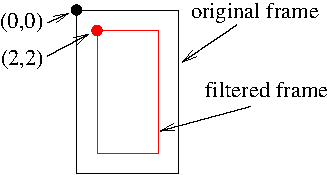
\includegraphics[scale=0.5]{filter}

\end{frame}
\begin{frame}[fragile]\frametitle{Indexing images}

Really bad:

\begin{Code}
  for (IntT x(0); x<576; ++x)  for (IntT y(0); y<720; ++y)
    im[x][y] += 3;
\end{Code}

\pause Slightly better:

\begin{Code}
  for (IntT x(0); x<im.Rows(); ++x)  for (IntT y(0); y<im.Cols(); ++y)
    im[x][y] += 3;
\end{Code}

\pause Better:

\begin{Code}
  for (IndexC x(im.TRow()); x<=im.BRow(); ++x)
    for (IndexC y(im.LCol()); y<=im.RCol(); ++y)
      im[x][y] += 3;
\end{Code}


\pause Best (and fastest):

\begin{Code}
  for (Array2dIterC<IntT>i(im); i; ++i)
    *i += 3;
\end{Code}

\end{frame}

\begin{frame}[fragile]\frametitle{Sliding one image around another} 

 The \Href{Class/RavlImageN.Rectangle2dIterC.html}{Rectangle2dIterC} iterator allows one image to scan over another larger one:\\\vfill

\centering{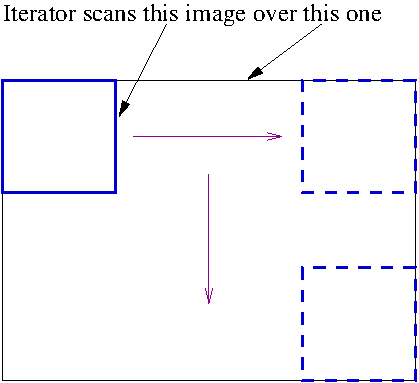
\includegraphics[scale=0.7]{slideim}}\\\vfill


 --- e.g. for image convolution
\end{frame}

\begin{frame}[fragile]\frametitle{Subimages}

Construct new image from old:

\begin{Code}
  ImageC<ByteT> a(576,720);
  a.Fill(12);
  ImageC<ByteT> b(a, IndexRange2dC(100,400,200,700));
  b.Fill(135);
\end{Code}

Data is {\em not} copied when constructing \Codebit{b}.  So \Codebit{a} finally is:

\centering{\vfill
\includegraphics[width=0.5\textwidth]{a}}

\end{frame}

\begin{frame}[fragile]\frametitle{Image I/O}

\Href{Tree/Ravl.API.Images.IO.html}{Image I/O using \Codebit{Load()} / \Codebit{Save()}}

\begin{itemize}
\item  can be files or devices
  (``\Href{Tree/Ravl.API.Images.IO.Virtual_Files.html}{virtual files}'')

\pause\item conversion between pixel types is automatic

 E.g. conversion of RGB 8-bit file to grey-scale float object:
\end{itemize}


\begin{Code}[commandchars=\\\{\}]
  #include "Ravl/IO.hh"
  #include "Ravl/Image/Image.hh"
  
  using namespace RavlN;
  using namespace RavlImageN;
  
  int main (int argc, char* argv[]) \{  
    ImageC<RealT> im;
    if (! Load ("image.png", im))    cerr << "panic!!" << endl;
    Save ("image.pgm", im);
    Save (\Href{Tree/Ravl.API.Graphics.Data_Display.html}{"@X:image"}, im); // write to screen with title "image"
  \} 
\end{Code}
  
\end{frame}


\begin{frame}[fragile]\frametitle{Image I/O (cont.)}

Corresponding {\tt defs.mk} file:\\[2em]

\begin{Code}
  MAINS= myprog.cc
  
  PROGLIBS = RavlImageIO RavlExtImgIO RavlDPDisplay
\end{Code}

\end{frame}

\begin{frame}[fragile]\frametitle{Video I/O}

Image sequence I/O --- to read and write a sequence:\\

\begin{Code}[commandchars=\\\{\}]
  #include "Ravl/DP/SequenceIO.hh"
  #include "Ravl/Image/Image.hh"
  #include "Ravl/Image/ByteRGBValue.hh"
  using namespace RavlN;
  using namespace RavlImageN;
  
  int main (int argc, char* argv[]) \{
    if (argc < 3)  exit(-1);
    DPIPortC<ImageC<ByteRGBValueC> > in;
    if(!OpenISequence(in, argv[1]))  exit(-2);
    DPOPortC<ImageC<ByteRGBValueC> > out;
    if(!OpenOSequence(out, argv[2])) exit (-3);
    ImageC<ByteRGBValueC> im;
    while(in.Get(im))
      out.Put(im);
  \}
\end{Code}
\end{frame}

\begin{frame}[fragile]\frametitle{Video I/O (cont.)}

~\\
Corresponding {\tt defs.mk} file:

\begin{Code}
  MAINS= seqio.cc

  PROGLIBS = RavlVideoIO RavlLibFFmpeg RavlDPDisplay
\end{Code}

\vfill\pause Run it like this to convert to sequence of `ppm's:

\begin{VerbatimXterm}
  seqio movie.mpeg tmp.ppm
\end{VerbatimXterm}

\vfill\pause Run it like this to display the file:

\begin{VerbatimXterm}[commandchars=\\\{\}]
  \Href{run:/vol/vssp/localsoft/External/linux/local/bin/runseqio}{seqio movie.mpeg @X}\footnote{\tiny To run this example, you need to (a) be using xpdf to run the presentation, (b) have compiled up the ``seqio'' example, and (c) have ``movie.mpeg'' in your current directory.\vfill}
\end{VerbatimXterm}

\vfill\pause Run it like this to display a camera o/p (include \Href{Tree/Ravl.API.Images.Video.Video_IO.Video4Linux.html}{RavlImgIOV4L} library):

\begin{VerbatimXterm}
  seqio @V4L @X
\end{VerbatimXterm}
\end{frame}


\begin{frame}[fragile]\frametitle{More general I/O}

Automatic numbering of file sequences:

\begin{itemize}
\item \Codebit{OpenOSequence(out,"a.ppm")} creates\\ a0.ppm, a1.ppm, ....,
  a10.ppm, ....

\pause\item \Codebit{OpenOSequence(out,"a\%4d.ppm")} creates\\ a0000.ppm, a0001.ppm, ....,
  a0010.ppm, ....
  
\pause\item \Codebit{OpenISequence(in,"a.ppm")} will read either style.

\pause\item \Codebit{Load()}, \Codebit{Save()}, \Codebit{OpenISequence}, \Codebit{OpenOSequence} can
  also be used for reading writing arbitrary objects (including images) as
  text files:

\begin{Code}
  ImageC<IntT>
  0 1 0 2
  32 35 45
  33 39 42
\end{Code}
\end{itemize}
\end{frame}


\section{Other classes etc.}

\begin{frame}[fragile]\frametitle{Graphics and GUIs}
  \centerline{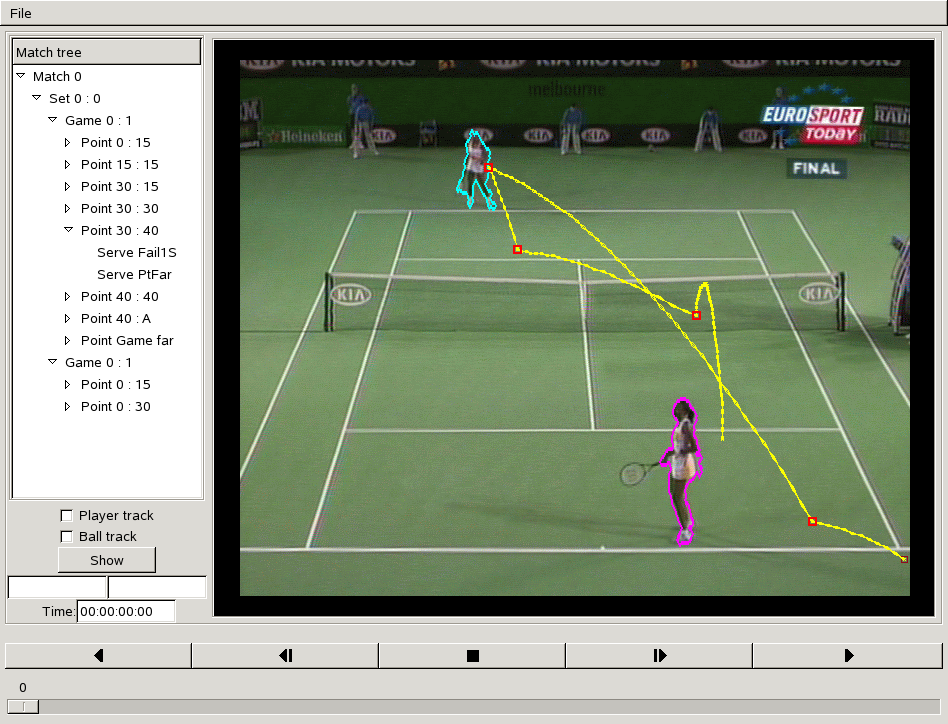
\includegraphics[height=\textheight,width=\textwidth,keepaspectratio]{tidyBrowser}}
\end{frame}

\begin{frame}[fragile]\frametitle{Maths}

  \begin{itemize}
  \item linear algebra
  \item Euclidean geometry
  \item projective geometry
    \begin{itemize}
    \item mosaicking:
      % \footnote{\tiny To run this example, you probably need to (a) be using xpdf to run the presentation and (b) have ``mosaic.mpeg'' in your current directory.  (Though I have done a hack for web users.)\vfill}
      %\Href{run:mplayer -loop 0 -x 600 -quiet mosaic.mpg}{\raisebox{-2.5ex}{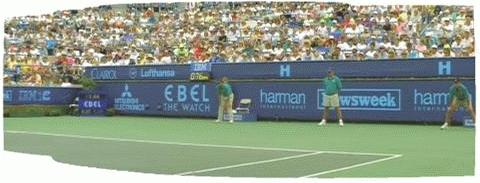
\includegraphics[width=0.3\textwidth]{mosaic}}}
      {\color{linkcolor} \setlength{\fboxrule}{1mm} \framebox{\raisebox{-3ex}{\movie[externalviewer]{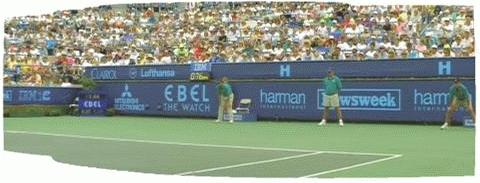
\includegraphics[width=0.3\textwidth]{mosaic}}{mosaic.mpg}}}}
    \end{itemize}
  \item ......
  \end{itemize}

\end{frame}

\begin{frame}[fragile]\frametitle{Pattern recognition}

  \Href{Tree/Ravl.API.Pattern_Recognition.Classifier.html}{Some standard classifiers:}

  \begin{itemize}
  \item SVM
  \item GMM
  \item ANN
  \item KNN
  \item ......
  \end{itemize}

Optimisers:

  \begin{itemize}
  \item conjugate gradient
  \item ......
  \end{itemize}

\end{frame}


\begin{frame}[fragile]\frametitle{O/S interfaces: threads}

  \begin{enumerate}
  \item Define the function to be launched as a thread, e.g.:

\begin{Code}
  bool PrintNumber(int &i) {
    cout << "PrintNumber called with value " << i << endl;
    return true;
  }
\end{Code}

  \item Create a ``\Href{Tree/Ravl.API.Core.Calls.html}{trigger}'': 

\begin{Code}
  TriggerC myTrigger = Trigger(&PrintNumber, 53);
\end{Code}

  \item Then launch it as a separate \Href{Class/RavlN.LaunchThreadC.html}{thread}:

\begin{Code}
  LaunchThreadC thread = LaunchThread (myTrigger) ; 
\end{Code}

\item and wait for it to finish:

\begin{Code}
  thread.Wait()
\end{Code}



\end{enumerate}
\end{frame}

\section{QMake}

\begin{frame}[fragile]\frametitle{QMake}

\centerline{\huge \Href{Tree/Ravl.QMake.html}{QMake}: a compilation tool}
\end{frame}

\begin{frame}[fragile]\frametitle{Compiling main programs}

  To compile (1 or more) main program(s) in a directory:
  \begin{itemize}
    \pause\item Create a file called \Codebit{defs.mk} in that directory,
    consisting of one line to tell QMake what the files are called:

\begin{Code}
  MAINS = main1.cc main2.cc main3.cc
\end{Code}

  \pause\item Execute the command \Codebit{qm}
  \end{itemize}

  \pause \vfill

  If your program(s) need RAVL libraries that QMake cannot find automatically
  at link time (mainly I/O libs), you will need to add them to the
  \Codebit{defs.mk} file.  E.g.:

\begin{Code}
  MAINS = main1.cc main2.cc main3.cc
  PROGLIBS = RavlVideoIO RavlLibFFmpeg RavlDPDisplay
\end{Code}
\end{frame}

\begin{frame}[fragile]\frametitle{Adding extra libraries}

  You can including your own class and header files:

  \vspace{2em}

\begin{Code}
  MAINS = main1.cc main2.cc main3.cc
  HEADERS = header1.hh header2.hh
  SOURCES = class1.cc class2.cc
\end{Code}

  \pause\vspace{2em}

  And \Href{Tree/Ravl.QMake.html}{much more...}
\end{frame}

\begin{frame}[fragile]\frametitle{Compiling with QMake}


  \begin{itemize}
  \pause\item {\tt qm} is just an alias for {\tt make}:
  \end{itemize}
\begin{VerbatimXterm}[fontsize=\tiny]
> alias qm 
gmake -f /vol/vssp/localsoft/Auto/linux/Ravl/share/RAVL/QMake/QMake.mk USERBUILD=1 !* && rehash
\end{VerbatimXterm}
  \vspace{-1.5ex}
  \begin{itemize}
  \pause\item For faster linking:
\begin{VerbatimXterm}
  qm shared
\end{VerbatimXterm}
    \pause\item For faster runtime:
\begin{VerbatimXterm}
  qm optshared
\end{VerbatimXterm}
    \pause\item Debugging using ddd / gdb:
\begin{VerbatimXterm}
  qm debugshared
\end{VerbatimXterm}
    \begin{itemize}
      \pause\item a bit of \Href{Tree/Ravl.Introduction.Debugging.html}{help in debugging RAVL}
      \pause\item \verb|qm shared|, \verb|qm debugshared| $\rightarrow$ run-time array bound checking
      
    \end{itemize}

    \pause\item {\tt \$PROJECT\_OUT}, {\tt /tmp/$<$user$>$/qm} can always be deleted:
\begin{VerbatimXterm}
  qm distclean
\end{VerbatimXterm}

  \end{itemize}
\end{frame}

\begin{frame}[fragile]\frametitle{Compiling with QMake (cont.)}

Static or shared (dynamic) libraries?

  \begin{itemize}
  \item static libs (use \Codebit{qm, qm debug, qm opt})\\
    -- good for long-running jobs (libs can't change)
  \pause\item shared libs (use \Codebit{qm shared, qm debugshared, qm optshared})\\
    -- good for development (fast linking)
  \end{itemize}

\vfill

    \pause ``Complete'' list of \Href{../../html/Help.txt}{{\tt qm} commands}:
\begin{VerbatimXterm}
  qm help
\end{VerbatimXterm}

\end{frame}


\section{Other bits}


\begin{frame}\frametitle{Documentation}

  \begin{itemize}
  \item \Href{index.html}{Class documentation} automatically generated from header files
  \pause\item Background documentation in \Href{Tree/Ravl.API.Images.html}{branches}, not in
    \Href{Class/RavlImageN.ImageC.html}{class leaves}\\[1em]

  \pause\item - while examples {\em are} usually in \Href{Class/RavlN.Array1dIterC.html}{class leaves}\\[1em]

  \pause\item \Href{Tree/Ravl.html}{Search engine}\\[1em]

  \pause \item 2 lots of documentation:
  \Href{http://vssp-www.ee.surrey.ac.uk/RavlInternal/RavlDoc/share/doc/RAVL/Auto/Basic/Tree/Ravl.html}{internal}, \Href{http://www.ee.surrey.ac.uk/Research/VSSP/Ravl/RavlIntro.html}{public}

  In each there is: 
  \begin{itemize}
  \pause \item  the \Href{Tree/Ravl.html}{blue users' version}, and
  \pause \item the \Href{../Develop/Tree/Ravl.html}{green developers' one}
  \end{itemize}

  \end{itemize}

\end{frame}

\begin{frame}[fragile]\frametitle{Finally....}


  \begin{itemize}

  \item Contributions always welcome (including C):
    \begin{itemize}
    \item for RAVL itself
    \item for use within CVSSP\\[1em]
    \end{itemize}
    \vfill
    \pause \item Go to
    \Href{http://www.ee.surrey.ac.uk/CVSSP/Ravl/RavlIntro.html}{http://www.ee.surrey.ac.uk/CVSSP/Ravl/RavlIntro.html}
    and read all about it.
    \vfill
    \setbeamercovered{transparent=3}
    \pause \item \color{red}\huge Tell us what is missing

  \end{itemize}
\end{frame}

\begin{frame}
 \color{code}\Huge\centerline{ We are here to help}
\end{frame}

\end{document}

\begin{frame}
  \pagecolor{titlebg} \thispagestyle{empty}
  \begin{center}
    \colorbox{titlebox}{\Huge\parbox{0.4\textwidth}{ \textcolor{titlecolor}{ \centering ~\\The end\\[1.2ex]}}}
  \end{center}
\end{frame}
